\subsection{Ostlo}
\subsubsection{Beholderkult}
I Ostlo smyger en grupp kultmedlemmar runt i skuggorna. De tillber \textit{Ögat}, en stor beholder som lever i katakomberna under staden. Kultmedlemmarna klär sig i röda dräkter med huvor, har rakade huvuden och ett öga tatuerat i pannan. Dessa spelas som en \textit{Cult Fanatic} \imagedescribe{\ref{img:cultFanatic}} ifrån Monster Manual \cite{MonsterManual}. De rör sig i gränder och mer laglösa värdshusen i Ostlo. De gillar att stjäla magiska föremål, specielt spelares arcane focus, och kan försöka stjäla dessa från spelarna.
%
\subsubsection{Ögat}
\begin{displayquote}
En mörkt marinblå klump svävar några decimeter över marken. Den har ett gigantiskt gult öga, en enorm mun med taggiga tänder och tentakler utstretande från sig med små ögon i ändarna.
\end{displayquote}
\textit{Ögat} är en beholder \imagedescribe{\ref{img:beholder}} som lever i katakomberna under Ostlo. Denna är ledaren för beholderkulten och samlar magiska artefakter i en hög bakom sig. Beholdern konverserar gärna med äventyrarna innan den anfaller dem, han är väldigt egosentrisk och har storhetsvansinne, och pratar främst om sig själv.

\begin{figure}
	\centering
	\label{img:cultFanatic}
	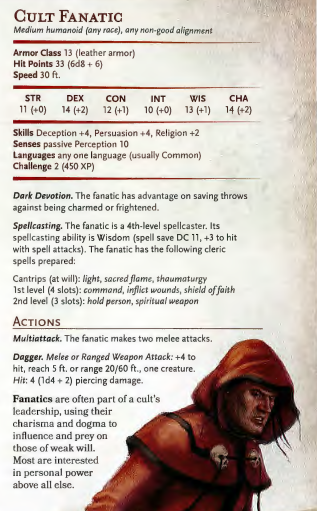
\includegraphics[width=\textwidth]{CultFanatic}
	\caption{\textit{Cult Fanatic} från \textit{Monster Manual D\&D 5e}\cite{MonsterManual}}
\end{figure}

\begin{figure}
	\centering
	\label{img:beholder}
	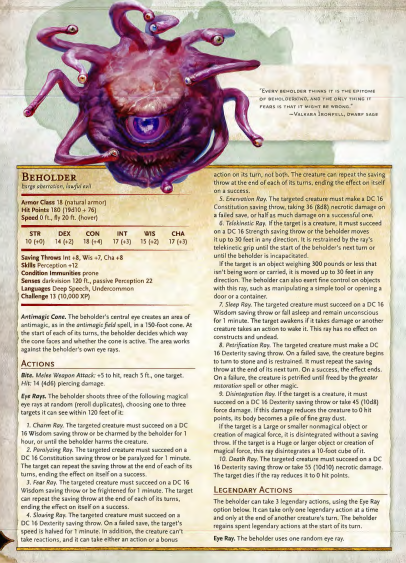
\includegraphics[width=\textwidth]{Beholder}
	\caption{\textit{Beholder} från \textit{Monster Manual D\&D 5e}\cite{MonsterManual}}
\end{figure}

\subsubsection{Katakomber under Ostlo}
Under Ostlo finns ett uråldrigt katatakombsystem. Detta var ursprungligen en kloak som användes av staden, men efter att detta fallit ur bruk har det tagits över av en Beholder som etablerat ett kultföljande. Följande rum finns i katakomberna.
%
\begin{enumerate}
	\item I en av de bredare kloakerna under Ostlo finns en ficka. Där finns en gammal port som är låst med ett stort gammalt lås. Bredvid sitter på var sida en slocknad fackla. Porten går att dyrka ganska lätt.
	\item 
	\item Här är en sovsal med tio våningssängar. Där finns även ett runt bord med stolar samt en eldstad. Det sitter tre kultister runt bordet samt tre i olika sängar. Alla utom två är beväpnade, men det finns vapen i rummet de kan hämta. Om man undersöker eldstaden kan man hitta en dold knapp, som öppnar en gång igenom eldstaden till en stege mot rum 10. För att gå igenom bör man släcka elden först. 
	\item Det här är den hemliga källaren under handelsboden Svarta Koftan. Det finns lagrat en del torkad mat, rep, facklor samt tre pilar i ett gammalt hölster.
	\item Det finns en stege ner till rum 9.
	\item En tänd fackla sitter mittemot gången mot rum 5. Om någon undersöker denna märker man att den går på ett gångjärn. Dras det i denna öppnas en hemlig dörr till rum 6. Där är det mörk, och det finns inga facklor där inne. Här finns en kista med 10 guld, 15 guld, 2 juveler. Det finns även en ringbrynja, en hjälm samt ett långsvärd.
	\item
	\item Igenom det här rummet rinner en flod kloakvatten, ner genom ett galler till rum 12. Gallret går att dra av och man kan ta sig igenom för varelser upp till liten storlek.
	\item 
	\item Här är en vinkällare. Det finns en kvast, 10 flaskor vin, 3 flaskor brännvin, 1 tunna mjöd, 10 limpor bröd samt 4 ostar. Går man upp mot rum 3 kan man skjuta upp den hemliga dörren, men det är svårt att ta sig ut om man inte lyckas få bort elden.
	\item 
	\item Här kommer det vatten från rum 8 till en liten pool med smutsigt vatten. I botten av polen ligger 3 kopparmynt. Polen flyter ut i en större kloak mot hamnen.
	\item Det här verkar vara någon form av skattkammare. Här finns en full tung rustning på en visningsdocka. Denna är i människostorlek, men kan modifieras enkelt till dvärgstorlek. Det finns 2 armborst, 20 armborst-boltar, två kortsvärd, en sköld, samt två kistor. En lista innehåller 3 sätt fina kläder och 3 munkdräkter. I den andra finns 15 guldmynt, 2 juveler och en liten ebonyststyett. 
	\item Det här är en stor sal med en upphöjd scen. På scenen flyter en stor Beholder. Denna är ledaren för kulten och samlar magiska artefakter i en hög bakom sig. Beholdern kallar sig ”Jag är” och konverserar gärna med äventyrarna innan den anfaller. Det finns även 3 kultister i salen som sjunger en hymn till Beholdern. Dessa anfaller med Beholdern.
\end{enumerate}
